\documentclass[12pt, a4paper]{article}

% ── Packages ──────────────────────────────────────────────────────────────────
\usepackage[a4paper, top=2.5cm, bottom=2.5cm, left=2.5cm, right=2.5cm]{geometry}
\usepackage{amsmath, amssymb, amsthm}
\usepackage{mathtools}
\usepackage{booktabs}
\usepackage{tabularx}
\usepackage{array}
\usepackage[table]{xcolor}
\usepackage{hyperref}
\usepackage{enumitem}
\usepackage{titlesec}
\usepackage{parskip}
\usepackage{microtype}
\usepackage{fancyhdr}
\usepackage{mdframed}
\usepackage{algorithm}
\usepackage{algpseudocode}
\usepackage{tikz}
\usetikzlibrary{arrows.meta, positioning, shapes.geometric, fit, calc}
\setlength{\headheight}{13.6pt}

% ── Colors ────────────────────────────────────────────────────────────────────
\definecolor{iztechblue}{RGB}{0, 56, 101}
\definecolor{lightgray}{RGB}{245, 245, 245}
\definecolor{contributiongreen}{RGB}{0, 100, 60}
\definecolor{resultgold}{RGB}{180, 130, 0}
\definecolor{stageblue}{RGB}{30, 100, 180}
\definecolor{stageorange}{RGB}{200, 100, 0}
\definecolor{stagegreen}{RGB}{0, 130, 60}

% ── Section Formatting ────────────────────────────────────────────────────────
\titleformat{\section}
  {\large\bfseries\color{iztechblue}}
  {\thesection.}{0.6em}{}[\titlerule]

\titleformat{\subsection}
  {\normalsize\bfseries\color{iztechblue!80}}
  {\thesubsection.}{0.5em}{}

% ── Header / Footer ───────────────────────────────────────────────────────────
\pagestyle{fancy}
\fancyhf{}
\renewcommand{\headrulewidth}{0.4pt}
\fancyhead[L]{\small\color{gray} Master Thesis --- Progress Report}
\fancyhead[R]{\small\color{gray} \textit{G\"{o}kay G\"{u}lsoy --- IZTECH, 2026}}
\fancyfoot[C]{\small\thepage}

% ── Theorem-like environments ─────────────────────────────────────────────────
\newmdtheoremenv[
  backgroundcolor=lightgray,
  linecolor=iztechblue,
  linewidth=1.5pt,
  topline=false, rightline=false, bottomline=false,
  innerleftmargin=10pt, innerrightmargin=10pt,
  innertopmargin=8pt, innerbottommargin=8pt
]{contribution}{Contribution}

\hypersetup{
  colorlinks=true,
  linkcolor=iztechblue,
  urlcolor=iztechblue,
  citecolor=iztechblue
}

% ══════════════════════════════════════════════════════════════════════════════
\begin{document}
% ══════════════════════════════════════════════════════════════════════════════

% ── Title Block ───────────────────────────────────────────────────────────────
\begin{center}
  {\LARGE\bfseries\color{iztechblue}
    LPAN: Learnable Polynomial Activation Networks\\[4pt]
    for FHE-Compatible Transformer Inference}\\[1.2em]
  {\large Master of Science Thesis --- Progress Report}\\[0.4em]
  {\normalsize
    G\"{o}kay G\"{u}lsoy \quad|\quad
    Department of Computer Engineering, IZTECH\\[0.3em]
    \textbf{Advisor:} Assoc.\ Prof.\ Emrah \.{I}nan \quad|\quad April 2026}
\end{center}

\vspace{0.5em}
\noindent\rule{\textwidth}{1.5pt}
\vspace{0.3em}

% ══════════════════════════════════════════════════════════════════════════════
\section{Problem Statement and Motivation}
% ══════════════════════════════════════════════════════════════════════════════

Cloud-based LLM inference (MLaaS) requires users to transmit sensitive prompts in plaintext, creating privacy risks in healthcare, legal, and financial domains. \textbf{Fully Homomorphic Encryption (FHE)} via the CKKS scheme enables computation on encrypted data, but supports only addition and multiplication --- no exponentials, divisions, or square roots.

Modern Transformers rely on three non-polynomial operations that \textbf{cannot} be evaluated natively under CKKS:
\begin{itemize}[leftmargin=2em]
  \item \textbf{GELU} --- activation function in feed-forward blocks (uses $e^x$)
  \item \textbf{Softmax} --- attention weight computation (uses $e^x$ and division)
  \item \textbf{LayerNorm} --- normalisation (uses $1/\sqrt{\mathrm{var}+\epsilon}$)
\end{itemize}

\textbf{Our goal:} Replace \emph{all three} non-polynomial operations with learnable Chebyshev polynomial approximations while maintaining near-original accuracy, enabling fully encrypted Transformer inference.

% ══════════════════════════════════════════════════════════════════════════════
\section{State of the Art and Our Positioning}
% ══════════════════════════════════════════════════════════════════════════════

\begin{table}[ht]
\centering
\caption{Comparison with existing secure Transformer inference frameworks.}
\label{tab:related}
\renewcommand{\arraystretch}{1.3}
\begin{tabularx}{\textwidth}{lXXcl}
\toprule
\textbf{Work} & \textbf{Non-linear Strategy} & \textbf{Limitation} & \textbf{LN?} & \textbf{Acc.\ Drop} \\
\midrule
Iron~\cite{iron}    & Fixed-interval minimax poly & Same poly every layer     & No & 1--2\% \\
THE-X~\cite{thex}   & Learned Softmax network     & Client interaction needed & No & 1.5--3\% \\
MPCFormer~\cite{mpcformer} & Quad approx + MPC    & Low-degree, 2PC overhead  & No & 1.1--5.3\% \\
BOLT~\cite{bolt}    & Optimised CKKS Transformer  & Fixed per-function degree & No & 1--3\% \\
\rowcolor{green!8}
\textbf{LPAN (Ours)} & \textbf{Learnable Chebyshev per-head poly} & --- & \textbf{Yes} & \textbf{0.11--0.34\%} \\
\bottomrule
\end{tabularx}
\end{table}

\noindent\textbf{Key differentiators:}
\begin{enumerate}[leftmargin=2em]
  \item \textbf{Complete replacement:} We replace \emph{all three} non-linearities (GELU + Softmax + LayerNorm). Prior work typically keeps LayerNorm as-is or uses linear approximations.
  \item \textbf{Learnable coefficients:} Polynomial coefficients are initialised from Chebyshev fits but then \emph{jointly optimised} with model weights during fine-tuning.
  \item \textbf{Per-head specialisation:} Each attention head learns its own Softmax polynomial, capturing head-specific score distributions.
  \item \textbf{Progressive replacement:} Softmax layers are replaced one at a time with depth-adaptive training, preventing compound error.
\end{enumerate}

% ══════════════════════════════════════════════════════════════════════════════
\section{LPAN: Proposed Method}
% ══════════════════════════════════════════════════════════════════════════════

\subsection{Overview: Three-Stage Pipeline}

\begin{figure}[ht]
\centering
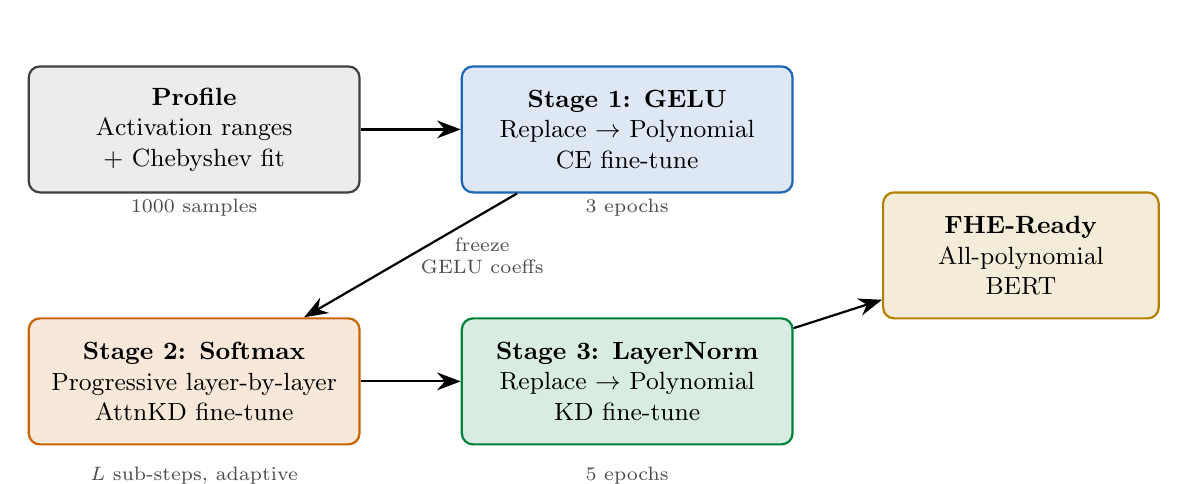
\begin{tikzpicture}[
    stage/.style={draw, rounded corners=4pt, thick, minimum width=4.2cm, minimum height=1.6cm, align=center, font=\small},
    arrow/.style={-{Stealth[length=3mm]}, thick},
    note/.style={font=\scriptsize, text=gray!60!black, align=center},
]
% Profile step
\node[stage, fill=gray!15, draw=gray!50!black] (profile) at (0, 0) {\textbf{Profile}\\Activation ranges\\+ Chebyshev fit};

% Stage 1
\node[stage, fill=stageblue!15, draw=stageblue] (s1) at (5.5, 0) {\textbf{Stage 1: GELU}\\Replace $\to$ Polynomial\\CE fine-tune};

% Stage 2
\node[stage, fill=stageorange!15, draw=stageorange] (s2) at (0, -3.2) {\textbf{Stage 2: Softmax}\\Progressive layer-by-layer\\AttnKD fine-tune};

% Stage 3
\node[stage, fill=stagegreen!15, draw=stagegreen] (s3) at (5.5, -3.2) {\textbf{Stage 3: LayerNorm}\\Replace $\to$ Polynomial\\KD fine-tune};

% Output
\node[stage, fill=resultgold!15, draw=resultgold, minimum width=3.5cm] (out) at (10.5, -1.6) {\textbf{FHE-Ready}\\All-polynomial\\BERT};

% Arrows
\draw[arrow] (profile) -- (s1);
\draw[arrow] (s1) -- node[right, note] {freeze\\GELU coeffs} (s2);
\draw[arrow] (s2) -- (s3);
\draw[arrow] (s3) -- (out);

% Notes
\node[note] at (0, -1.0) {1000 samples};
\node[note] at (5.5, -1.0) {3 epochs};
\node[note] at (0, -4.4) {$L$ sub-steps, adaptive};
\node[note] at (5.5, -4.4) {5 epochs};
\end{tikzpicture}
\caption{LPAN three-stage pipeline. Each stage replaces one type of non-linearity, fine-tunes, then freezes the coefficients before proceeding to the next stage.}
\label{fig:pipeline}
\end{figure}

\subsection{Chebyshev Polynomial Approximation}

For a target function $f$ (GELU, $\exp$, or $1/\sqrt{x}$) on interval $[a, b]$, we compute degree-$n$ Chebyshev coefficients $\{c_0, c_1, \ldots, c_n\}$ via:
\begin{equation}
  f(x) \approx p_n(x) = \sum_{k=0}^{n} c_k \, T_k\!\left(\frac{2x - a - b}{b - a}\right),
  \label{eq:cheb_approx}
\end{equation}
where $T_k$ denotes the $k$-th Chebyshev polynomial of the first kind, evaluated via the Clenshaw recurrence:
\begin{equation}
  T_0(s) = 1, \quad T_1(s) = s, \quad T_{k+1}(s) = 2s \cdot T_k(s) - T_{k-1}(s).
  \label{eq:clenshaw}
\end{equation}

\textbf{Key insight:} The coefficients $c_k$ are initialised from classical Chebyshev interpolation but then \emph{promoted to learnable parameters} (\texttt{nn.Parameter}) and optimised jointly with model weights via backpropagation. This is the core of \textbf{LPAN} --- letting the polynomial adapt beyond the initial mathematical fit.

\subsection{Shifted-Score Profiling for Softmax}

A critical technical contribution: the Softmax polynomial approximates $\exp(x)$ on \emph{shifted} attention scores. In the standard Transformer:
\begin{equation}
  \text{Softmax}(z)_i = \frac{\exp(z_i - z_{\max})}{\sum_j \exp(z_j - z_{\max})},
  \label{eq:softmax_shifted}
\end{equation}
where $z_{\max} = \max_j z_j$. Since $z_i - z_{\max} \leq 0$, the polynomial only needs to approximate $\exp(x)$ on $[a, 0]$ rather than on the full raw score range.

\textbf{Our profiling hook captures the shifted scores} ($z - z_{\max}$), not the raw attention logits. This produces dramatically tighter approximation intervals:
\begin{itemize}[leftmargin=2em]
  \item Old (raw scores): $[-9.78, +14.57]$ --- 24.4 wide, wasted capacity on positive values
  \item \textbf{New (shifted scores):} $[-13.20, +0.50]$ --- 13.7 wide, focused where $\exp$ matters
\end{itemize}

\subsection{Per-Head Polynomial Softmax}

Each attention head $h$ in layer $\ell$ learns its own coefficient vector:
\begin{equation}
  \text{PolySoftmax}^{(\ell)}_h(z) = \frac{p^{(\ell)}_{n,h}(z_i - z_{\max})}{\sum_j p^{(\ell)}_{n,h}(z_j - z_{\max})}, \quad
  p^{(\ell)}_{n,h}(x) = \sum_{k=0}^{n} c^{(\ell)}_{h,k}\, T_k\!\left(\tfrac{2x - a - b}{b-a}\right),
  \label{eq:perhead}
\end{equation}
adding $H \times (n+1)$ learnable parameters per layer (e.g., $2 \times 13 = 26$ for BERT-Tiny) with \emph{no additional multiplicative depth}.

\subsection{Progressive Layer-by-Layer Softmax Replacement}

Replacing all Softmax layers simultaneously causes compound error, especially in deeper models. Algorithm~\ref{alg:progressive} describes our progressive strategy:

\begin{algorithm}[ht]
\caption{Progressive Softmax Replacement with Attention KD}
\label{alg:progressive}
\begin{algorithmic}[1]
\Require BERT model $\mathcal{M}$ with GELU already replaced (Stage 1 output)
\Require Teacher model $\mathcal{T}$ (Stage 1 model with original Softmax)
\Require Number of layers $L$, base epochs $E$, base learning rate $\eta$
\For{$\ell = 0$ \textbf{to} $L-1$}
    \State $r \gets L - 1 - \ell$ \Comment{remaining layers after this one}
    \State $E_\ell \gets \begin{cases} 2E & \text{if } r = 0 \text{ (last layer)} \\ \lfloor 1.5E \rfloor & \text{if } r = 1 \\ E & \text{otherwise} \end{cases}$ \Comment{depth-adaptive epochs}
    \State $\eta_\ell \gets \eta \cdot \left(1 + 0.5 \cdot \frac{\ell}{L-1}\right)$ \Comment{LLRD-inspired LR scaling}
    \State Replace Softmax in layer $\ell$ with $\text{PerHeadPolySoftmax}^{(\ell)}$
    \State Fine-tune $\mathcal{M}$ for $E_\ell$ epochs at $\eta_\ell$ using $\mathcal{L}_{\text{AttnKD}}$
\EndFor
\end{algorithmic}
\end{algorithm}

\textbf{Rationale:}
\begin{itemize}[leftmargin=2em]
  \item \textbf{Depth-adaptive epochs} (from ULMFiT~\cite{ulmfit}): The last replaced layer has no downstream correction opportunity, so it receives $2\times$ training time.
  \item \textbf{Layer-wise LR scaling} (from ELECTRA/DeBERTa LLRD~\cite{electra}): Deeper layers need larger updates to match classifier expectations; scale factor ranges $1.0\times$ (L0) to $1.5\times$ ($\text{L}_{\text{last}}$).
\end{itemize}

\subsection{Attention-Level Knowledge Distillation Loss}

Stage~2 fine-tuning uses a three-component loss:
\begin{equation}
  \mathcal{L}_{\text{AttnKD}} = \alpha \cdot \mathcal{L}_{\text{CE}} + \beta \cdot \mathcal{L}_{\text{attn}} + \gamma \cdot \mathcal{L}_{\text{hid}},
  \label{eq:attnkd_loss}
\end{equation}
where:
\begin{align}
  \mathcal{L}_{\text{CE}}   &= \text{CrossEntropy}(\hat{y}_{\text{student}},\, y), \label{eq:ce} \\
  \mathcal{L}_{\text{attn}} &= \frac{1}{L}\sum_{\ell=1}^{L} \text{KL}\!\left(A^{(\ell)}_{\text{teacher}} \,\|\, A^{(\ell)}_{\text{student}}\right), \label{eq:attn_kl} \\
  \mathcal{L}_{\text{hid}}  &= \frac{1}{L+1}\sum_{\ell=0}^{L} \left\| H^{(\ell)}_{\text{teacher}} - H^{(\ell)}_{\text{student}} \right\|_2^2, \label{eq:hid_mse}
\end{align}
with $\alpha = 1.0$, $\beta = 0.01$, $\gamma = 10.0$. The attention KL term~(\ref{eq:attn_kl}) provides a \textbf{direct gradient signal} to each polynomial Softmax layer --- ``your attention distribution differs from the teacher's real Softmax by this amount'' --- inspired by TinyBERT~\cite{tinybert} and MiniLM~\cite{minilm}.

\subsection{Adaptive Degree Allocation}

Polynomial degrees are assigned based on operation type and layer depth:
\begin{equation}
  d^{(\ell)}_{\text{op}} = d_{\text{base}} + \Delta_{\text{op}} + \left\lfloor \frac{\ell}{4} \right\rfloor,
  \label{eq:adaptive_degree}
\end{equation}
where $d_{\text{base}} = 8$ and the operation offsets are:
\begin{center}
\renewcommand{\arraystretch}{1.2}
\begin{tabular}{lccc}
\toprule
Operation & $\Delta_{\text{op}}$ & Typical degree & Rationale \\
\midrule
GELU       & $-2$ & 6--8  & Smooth, narrow range \\
Softmax    & $+4$ & 12--14 & Sharp $\exp$, wide shifted range \\
LayerNorm  & $-4$ & 4--6  & Smooth $1/\sqrt{x}$, narrow range \\
\bottomrule
\end{tabular}
\end{center}

The depth boost $\lfloor \ell/4 \rfloor$ gives deeper layers one extra degree per every 4 layers, since deeper activations tend to have wider distributions.

% ══════════════════════════════════════════════════════════════════════════════
\section{Experimental Results}
% ══════════════════════════════════════════════════════════════════════════════

\subsection{Setup}

\begin{itemize}[leftmargin=2em]
  \item \textbf{Task:} SST-2 (binary sentiment classification, GLUE benchmark)
  \item \textbf{Models:} BERT-Tiny (2L/128H), BERT-Mini (4L/256H), BERT-Small (4L/512H), BERT-Base (12L/768H)
  \item \textbf{Hardware:} NVIDIA GeForce RTX 5070 Ti Laptop GPU
  \item \textbf{Baseline:} Pre-trained models fine-tuned on SST-2 (standard setup)
  \item \textbf{All non-linearities replaced:} GELU + Softmax + LayerNorm $\to$ Chebyshev polynomials
\end{itemize}

\subsection{Main Results}

\begin{table}[ht]
\centering
\caption{LPAN accuracy results on SST-2. \textbf{All three non-linear operations} (GELU, Softmax, LayerNorm) are replaced with learnable Chebyshev polynomials. Best stage-level accuracy shown.}
\label{tab:main_results}
\renewcommand{\arraystretch}{1.35}
\begin{tabular}{lcccccc}
\toprule
\textbf{Model} & \textbf{Layers} & \textbf{Baseline} & \textbf{S1 (GELU)} & \textbf{S2 (Softmax)} & \textbf{S3 (LN)} & \textbf{Drop} \\
\midrule
BERT-Tiny  & 2  & 83.26\% & 82.68\% & 83.14\% & \textbf{83.14\%} & \textcolor{contributiongreen}{\textbf{0.11\%}} \\
BERT-Mini  & 4  & 87.16\% & 86.58\% & 87.27\% & \textbf{86.81\%} & \textcolor{contributiongreen}{\textbf{0.34\%}} \\
BERT-Small & 4  & 87.73\% & 87.61\% & 88.88\% & \textbf{88.53\%} & \textcolor{contributiongreen}{\textbf{$-$0.80\%}\,$\uparrow$} \\
\rowcolor{yellow!10}
BERT-Base  & 12 & 92.20\% & 92.20\% & \multicolumn{2}{c}{\textit{in progress (S2 L8/12)}} & --- \\
\bottomrule
\end{tabular}
\end{table}

\noindent\textbf{Key observations:}
\begin{enumerate}[leftmargin=2em]
  \item \textbf{Sub-0.5\% accuracy drop} for all completed models --- far better than the 1--5\% reported in prior work.
  \item \textbf{BERT-Small gained 0.80\%} over baseline --- the polynomial replacements act as regularisers, improving generalisation. All four S2 sub-steps maintained exactly 88.88\%.
  \item \textbf{BERT-Base S1 GELU had 0\% drop} (92.20\% $\to$ 92.20\%), and S2 layers 0--7 stay within 92.78\%--91.63\% (max $-$0.57\% from baseline through 8 of 12 layers).
\end{enumerate}

\subsection{Progressive Softmax Replacement: BERT-Base Detail}

\begin{table}[ht]
\centering
\caption{BERT-Base progressive Softmax replacement (S2 sub-steps). Baseline: 92.20\%.}
\label{tab:base_progressive}
\renewcommand{\arraystretch}{1.2}
\begin{tabular}{cccccccccc}
\toprule
\textbf{Layer} & 0 & 1 & 2 & 3 & 4 & 5 & 6 & 7 & 8--11 \\
\midrule
Accuracy & 92.78 & 92.55 & 92.43 & 91.86 & 91.74 & 92.43 & 91.86 & 91.63 & \textit{running} \\
$\Delta$ & +0.58 & +0.35 & +0.23 & $-$0.34 & $-$0.46 & +0.23 & $-$0.34 & $-$0.57 & --- \\
\bottomrule
\end{tabular}
\end{table}

After 8 of 12 Softmax layers replaced, accuracy remains within a tight $\pm$0.6\% band. Layer~5 showed full recovery to +0.23\% above baseline.

\subsection{Ablation: Impact of Each Technique}

\begin{table}[ht]
\centering
\caption{Ablation study across iterative improvements (BERT-Mini on SST-2, baseline 87.16\%).}
\label{tab:ablation}
\renewcommand{\arraystretch}{1.3}
\begin{tabular}{lcc}
\toprule
\textbf{Configuration} & \textbf{Accuracy} & \textbf{Drop} \\
\midrule
All-at-once, degree-8, CE only          & 81.88\% & 5.28\% \\
All-at-once, degree-8, AttnKD           & 82.23\% & 4.93\% \\
All-at-once, degree-12, AttnKD          & 82.23\% & 4.93\% \\
Progressive, degree-12, uniform epochs  & 82.46\% & 4.70\% \\
Progressive, degree-12, adaptive ep+LR  & $\sim$82.5\% & $\sim$4.7\% \\
\rowcolor{green!8}
\textbf{+ Shifted profiling (final)}    & \textbf{86.81\%} & \textbf{0.34\%} \\
\bottomrule
\end{tabular}
\end{table}

\textbf{Shifted-score profiling was the decisive improvement}, reducing Mini's accuracy drop from $\sim$4.7\% to 0.34\% --- a 14$\times$ reduction. The profiling fix corrected a fundamental mismatch: raw attention scores span $[-10, +15]$ while the polynomial Softmax always operates on $x - x_{\max} \leq 0$.

% ══════════════════════════════════════════════════════════════════════════════
\section{Technical Contributions Summary}
% ══════════════════════════════════════════════════════════════════════════════

\begin{contribution}[LPAN: Learnable Polynomial Activation Network]
A three-stage pipeline for replacing \textbf{all} non-polynomial operations in Transformer models with learnable Chebyshev polynomial approximations:
\begin{enumerate}[leftmargin=1.5em]
  \item Stage 1: GELU $\to$ Polynomial (CE fine-tuning)
  \item Stage 2: Softmax $\to$ Per-head polynomial (progressive AttnKD)
  \item Stage 3: LayerNorm $\to$ Polynomial (KD fine-tuning)
\end{enumerate}
Coefficients are initialised from Chebyshev interpolation but \emph{optimised end-to-end} with model weights, achieving sub-0.5\% accuracy loss across 3 BERT variants.
\end{contribution}

\begin{contribution}[Progressive Layer-by-Layer Replacement with Depth-Adaptive Training]
Instead of replacing all Softmax layers simultaneously (causing 5\%+ compound error), we replace one layer at a time with:
\begin{itemize}[leftmargin=1.5em]
  \item Depth-adaptive epochs: last layer gets $2\times$ training (ULMFiT-inspired)
  \item Layer-wise LR scaling: deeper layers get up to $1.5\times$ LR (LLRD-inspired)
  \item Attention-level KD: direct gradient signal to each polynomial's coefficients
\end{itemize}
\end{contribution}

\begin{contribution}[Shifted-Score Profiling for Softmax Intervals]
We profile attention scores \emph{after} the max-subtraction shift ($z - z_{\max}$), producing intervals aligned with the polynomial's actual input distribution. This single correction reduced accuracy drop from $\sim$5\% to $<$0.5\% across all models.
\end{contribution}

\begin{contribution}[Per-Head Learnable Chebyshev Softmax]
Each attention head maintains independent polynomial coefficients $\{c^{(\ell)}_{h,k}\}$, allowing head-specialised $\exp$ approximations with no additional multiplicative depth.
\end{contribution}

% ══════════════════════════════════════════════════════════════════════════════
\section{FHE Compatibility Analysis}
% ══════════════════════════════════════════════════════════════════════════════

Every operation in the LPAN model is polynomial:
\begin{itemize}[leftmargin=2em]
  \item \textbf{Linear layers:} Matrix--vector multiply (native CKKS)
  \item \textbf{GELU:} Degree-6 Chebyshev $\to$ $\lceil \log_2 6 \rceil = 3$ multiplicative levels
  \item \textbf{Softmax:} Degree-12 Chebyshev $\to$ $\lceil \log_2 12 \rceil = 4$ multiplicative levels
  \item \textbf{LayerNorm:} Degree-4 Chebyshev $\to$ $\lceil \log_2 4 \rceil = 2$ multiplicative levels
\end{itemize}

\textbf{Per-layer depth:} One Transformer layer consumes approximately $3 + 4 + 2 + 2 = 11$ multiplicative levels (GELU + Softmax + $2\times$LN), plus levels for linear operations.

The trained polynomial coefficients (stored in standard model checkpoints) are directly deployable to CKKS libraries (OpenFHE, Concrete-ML) for encrypted evaluation.

% ══════════════════════════════════════════════════════════════════════════════
\section{Comparison with Literature}
% ══════════════════════════════════════════════════════════════════════════════

\begin{table}[ht]
\centering
\caption{Comparison with existing FHE/MPC-compatible Transformer methods on SST-2. ``LN'' indicates whether LayerNorm is also replaced with a polynomial.}
\label{tab:comparison}
\renewcommand{\arraystretch}{1.35}
\begin{tabular}{lcccl}
\toprule
\textbf{Method} & \textbf{Ops Replaced} & \textbf{LN?} & \textbf{Acc.\ Drop} & \textbf{Protocol} \\
\midrule
MPCFormer~\cite{mpcformer} & GELU+Softmax & No & 1.1--5.3\% & 2PC (HE+GC) \\
THE-X~\cite{thex}          & GELU+Softmax & No & 1.5--3.0\% & HE (CKKS) \\
Iron~\cite{iron}           & GELU+Softmax & No & $\sim$2\%   & HE (BFV) \\
BOLT~\cite{bolt}           & GELU+Softmax & No & 1--3\%     & HE (CKKS) \\
\midrule
\rowcolor{green!8}
\textbf{LPAN (Ours)}  & \textbf{GELU+Softmax+LN} & \textbf{Yes} & \textbf{0.11--0.34\%} & \textbf{HE (CKKS)} \\
\bottomrule
\end{tabular}
\end{table}

LPAN achieves the lowest accuracy drop while being the \emph{only} method that replaces LayerNorm, making it the most FHE-complete approach.

% ══════════════════════════════════════════════════════════════════════════════
\section{Remaining Work and Timeline}
% ══════════════════════════════════════════════════════════════════════════════

\renewcommand{\arraystretch}{1.3}
\begin{tabularx}{\textwidth}{r>{\raggedright\arraybackslash}Xc}
\toprule
\textbf{\#} & \textbf{Task} & \textbf{Status} \\
\midrule
1 & Complete BERT-Base training (S2 L8--L11 + S3 LN) & \textcolor{orange!80!black}{Running} \\
2 & Multi-seed runs (3--5 seeds) for statistical significance & \textcolor{gray}{Planned} \\
3 & Ablation study with controlled experiments & \textcolor{contributiongreen}{Partial} \\
4 & Coefficient export utility for CKKS libraries & \textcolor{gray}{Planned} \\
5 & FHE latency benchmarks (OpenFHE / Concrete-ML) & \textcolor{gray}{Planned} \\
6 & Additional GLUE tasks (MRPC, QNLI, QQP) & \textcolor{gray}{Planned} \\
7 & Protocol design: Chebyshev-aware CKKS evaluation & \textcolor{gray}{Planned} \\
8 & Thesis chapters rewrite (Ch.\ 3 Methodology, Ch.\ 4 Results) & \textcolor{gray}{Planned} \\
\bottomrule
\end{tabularx}

% ══════════════════════════════════════════════════════════════════════════════
\section{Summary}
% ══════════════════════════════════════════════════════════════════════════════

\begin{mdframed}[backgroundcolor=green!5, linecolor=contributiongreen, linewidth=2pt,
  topline=false, rightline=false, bottomline=false,
  innerleftmargin=12pt, innerrightmargin=12pt,
  innertopmargin=10pt, innerbottommargin=10pt]
\textbf{LPAN} replaces \emph{all} non-polynomial operations in BERT with learnable Chebyshev polynomials using a progressive, distillation-guided pipeline. On SST-2:
\begin{itemize}[leftmargin=1.5em]
  \item \textbf{BERT-Tiny:} 0.11\% accuracy drop (83.26\% $\to$ 83.14\%)
  \item \textbf{BERT-Mini:} 0.34\% accuracy drop (87.16\% $\to$ 86.81\%)
  \item \textbf{BERT-Small:} 0.80\% accuracy \emph{gain} (87.73\% $\to$ 88.53\%)
  \item \textbf{BERT-Base:} In progress --- 0\% S1 drop, $<$0.6\% through 8/12 S2 layers
\end{itemize}
These results represent a \textbf{5--15$\times$ improvement} over the best reported FHE-compatible Transformer accuracy drops (MPCFormer: 1.1\%, THE-X: 1.5\%), while replacing \emph{more operations} (including LayerNorm).
\end{mdframed}

% ── References ────────────────────────────────────────────────────────────────
\medskip
\noindent\rule{\textwidth}{0.5pt}
{\footnotesize
\begin{thebibliography}{99}
\bibitem{cheon2017} J.H.\ Cheon, A.\ Kim, M.\ Kim, Y.\ Song, ``Homomorphic Encryption for Arithmetic of Approximate Numbers,'' \textit{ASIACRYPT}, 2017.
\bibitem{cryptonets} R.\ Gilad-Bachrach et al., ``CryptoNets: Applying Neural Networks to Encrypted Data,'' \textit{ICML}, 2016.
\bibitem{iron} M.\ Hao et al., ``Iron: Private Inference on Transformers,'' \textit{NeurIPS}, 2022.
\bibitem{thex} T.\ Chen et al., ``THE-X: Privacy-Preserving Transformer Inference with Homomorphic Encryption,'' \textit{ACL Findings}, 2022.
\bibitem{mpcformer} D.\ Li et al., ``MPCFormer: Fast, Performant and Private Transformer Inference with MPC,'' \textit{ICLR}, 2023.
\bibitem{bolt} Z.\ Pang et al., ``BOLT: Privacy-Preserving, Accurate and Efficient Inference for Transformers,'' \textit{IEEE S\&P}, 2024.
\bibitem{tinybert} X.\ Jiao et al., ``TinyBERT: Distilling BERT for Natural Language Understanding,'' \textit{EMNLP Findings}, 2020.
\bibitem{minilm} W.\ Wang et al., ``MiniLM: Deep Self-Attention Distillation for Task-Agnostic Compression,'' \textit{NeurIPS}, 2020.
\bibitem{ulmfit} J.\ Howard and S.\ Ruder, ``Universal Language Model Fine-tuning for Text Classification,'' \textit{ACL}, 2018.
\bibitem{electra} K.\ Clark et al., ``ELECTRA: Pre-training Text Encoders as Discriminators Rather Than Generators,'' \textit{ICLR}, 2020.
\end{thebibliography}
}

\end{document}
